\documentclass{article}\usepackage[]{graphicx}\usepackage[]{color}
%% maxwidth is the original width if it is less than linewidth
%% otherwise use linewidth (to make sure the graphics do not exceed the margin)
\makeatletter
\def\maxwidth{ %
  \ifdim\Gin@nat@width>\linewidth
    \linewidth
  \else
    \Gin@nat@width
  \fi
}
\makeatother

\definecolor{fgcolor}{rgb}{0.345, 0.345, 0.345}
\newcommand{\hlnum}[1]{\textcolor[rgb]{0.686,0.059,0.569}{#1}}%
\newcommand{\hlstr}[1]{\textcolor[rgb]{0.192,0.494,0.8}{#1}}%
\newcommand{\hlcom}[1]{\textcolor[rgb]{0.678,0.584,0.686}{\textit{#1}}}%
\newcommand{\hlopt}[1]{\textcolor[rgb]{0,0,0}{#1}}%
\newcommand{\hlstd}[1]{\textcolor[rgb]{0.345,0.345,0.345}{#1}}%
\newcommand{\hlkwa}[1]{\textcolor[rgb]{0.161,0.373,0.58}{\textbf{#1}}}%
\newcommand{\hlkwb}[1]{\textcolor[rgb]{0.69,0.353,0.396}{#1}}%
\newcommand{\hlkwc}[1]{\textcolor[rgb]{0.333,0.667,0.333}{#1}}%
\newcommand{\hlkwd}[1]{\textcolor[rgb]{0.737,0.353,0.396}{\textbf{#1}}}%

\usepackage{framed}
\makeatletter
\newenvironment{kframe}{%
 \def\at@end@of@kframe{}%
 \ifinner\ifhmode%
  \def\at@end@of@kframe{\end{minipage}}%
  \begin{minipage}{\columnwidth}%
 \fi\fi%
 \def\FrameCommand##1{\hskip\@totalleftmargin \hskip-\fboxsep
 \colorbox{shadecolor}{##1}\hskip-\fboxsep
     % There is no \\@totalrightmargin, so:
     \hskip-\linewidth \hskip-\@totalleftmargin \hskip\columnwidth}%
 \MakeFramed {\advance\hsize-\width
   \@totalleftmargin\z@ \linewidth\hsize
   \@setminipage}}%
 {\par\unskip\endMakeFramed%
 \at@end@of@kframe}
\makeatother

\definecolor{shadecolor}{rgb}{.97, .97, .97}
\definecolor{messagecolor}{rgb}{0, 0, 0}
\definecolor{warningcolor}{rgb}{1, 0, 1}
\definecolor{errorcolor}{rgb}{1, 0, 0}
\newenvironment{knitrout}{}{} % an empty environment to be redefined in TeX

\usepackage{alltt}
\usepackage[letterpaper, portrait, margin=1in]{geometry}
\usepackage{amsmath}

\title{Math 680 - Assignment \#2}
\author{Kevin McGregor}
\date{October 15th, 2015}
\IfFileExists{upquote.sty}{\usepackage{upquote}}{}
\begin{document}
\maketitle

\section*{Question 1}
We're trying to minimize $\|Y-X\beta\|^2$ with respect to $\beta$.  We know that the least squares criterion is a convex function, therefore the minimum we find will be a global minimum.  The function can be rewritten as:

\begin{eqnarray*}
  \|Y-X\beta\|^2 &=& (Y-X\beta)^\top(Y-X\beta) \\
                 &=& Y^\top Y - (X\beta)^\top Y - Y^\top X\beta + (X\beta)^\top X\beta \\
                 &=& Y^\top Y - 2(X\beta)^\top Y + \beta^\top X^\top X\beta.
\end{eqnarray*}

Then, differentiating with respect to $\beta$ gives:

\begin{eqnarray*}
  \nabla_\beta \|Y-X\beta\|^2 &=& -2X^\top Y + 2X^\top X\beta.
\end{eqnarray*}

So, if we plug in the centered least squares estimate for $\beta$ into this equation, we know it will be a global minimum for the least squares criterion.

WILL COME BACK TO THIS!

\section*{Question 2}
\subsection*{(a)}
\begin{eqnarray*}
  \|\tilde{Y}-\tilde{X}\beta\|^2 + \lambda\|\beta\|^2 &=& (\tilde{Y}-\tilde{X}\beta)^\top(\tilde{Y}-\tilde{X}\beta) + \lambda\beta^\top\beta \\
                 &=& \tilde{Y}^\top\tilde{Y} - 2\beta^\top\tilde{X}^\top\tilde{Y} + \beta^\top\tilde{X}^\top\tilde{X}\beta + \lambda\beta^\top\beta \\
 \nabla f(\beta) &=& -2\tilde{X}^\top\tilde{Y} + 2\tilde{X}^\top\tilde{X}\beta + 2\lambda\beta
\end{eqnarray*}

\subsection*{(b)}
The function $f$ is quadratic in $\beta$, and the matrix in the quadratic term is $\tilde{X}^\top\tilde{X}+\lambda I$, which is positive definite.  Therefore $f$ is strictly convex.

\subsection*{(c)}
Since $f$ is strictly convex, there is only one global minimizer of $f$.

\subsection*{(d)}
See R code in ``a2\_q2d.R'' and ``centeredRidge\_func.R''

\subsection*{(e)}
The solution to ridge regression is found by setting $\nabla f(\beta)=0$, which gives us $\hat{\beta}^{(\lambda)}_{-1}=(\tilde{X}^\top\tilde{X}+\lambda I)^{-1}\tilde{X}^\top\tilde{Y}$.  So we have the expected value:

\begin{eqnarray*}
  E[\hat{\beta}^{(\lambda)}_{-1}] &=& E[(\tilde{X}^\top\tilde{X}+\lambda I)^{-1}\tilde{X}^\top\tilde{Y}] \\
            &=& (\tilde{X}^\top\tilde{X}+\lambda I)^{-1}\tilde{X}^\top E[\tilde{Y}] \\
            &=&  (\tilde{X}^\top\tilde{X}+\lambda I)^{-1}\tilde{X}^\top\tilde{X}\beta_{*-1},
\end{eqnarray*}
and the variance:

\begin{eqnarray*}
  var[\hat{\beta}^{(\lambda)}_{-1}] &=& var[(\tilde{X}^\top\tilde{X}+\lambda I)^{-1}\tilde{X}^\top\tilde{Y}] \\
            &=& [(\tilde{X}^\top\tilde{X}+\lambda I)^{-1}\tilde{X}^\top] var[\tilde{Y}] [(\tilde{X}^\top\tilde{X}+\lambda I)^{-1}\tilde{X}^\top]^\top \\
            &=& \sigma^2_* [(\tilde{X}^\top\tilde{X}+\lambda I)^{-1}\tilde{X}^\top ] [(\tilde{X}^\top\tilde{X}+\lambda I)^{-1}\tilde{X}^\top]^\top,
\end{eqnarray*}
since $var[\tilde{Y}]=\sigma^2_* I$.

\vspace{0.5in}

In the simulation study, we independently generate $Y$ 1000 times.  The R code for this can be seen in the file ``a2\_q2d.R''. Figure~\ref{fig:q2_graphs} plots the theoretical vs. observed expectation and variance (i.e. the individual elements of each vector or matrix).  Since most points fall close to the diagonal, the observed expectation and variance were close to the theoretical values.


\begin{knitrout}
\definecolor{shadecolor}{rgb}{0.969, 0.969, 0.969}\color{fgcolor}\begin{figure}
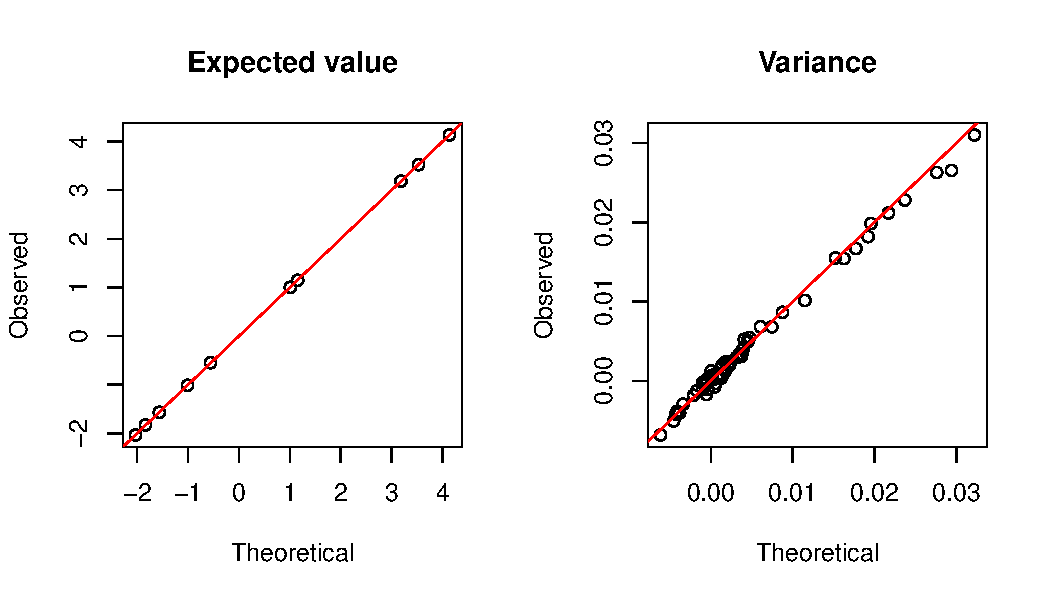
\includegraphics[width=\maxwidth]{figure/q2_graphs-1} \caption[Observed vs]{Observed vs. Theoretical Expectation and Variance for the centered ridge estimator}\label{fig:q2_graphs}
\end{figure}


\end{knitrout}


\section*{Question 3}
See R code in ``ridge\_crossval.R''.

\section*{Question 4}
The simulation setup and top-level function (ridgeSim) are in the file ``a2\_q4.R''.  The function ridgeSim also calls functions from the files ``centeredRidge\_func.R'' and ``ridge\_crossval.R''.  It calculates the singular value decomposition only once, then selects the proper rows for each iteration of the cross-validation step. 

\begin{table}[!htb]
    \caption{Losses for the various simulation scenarios when $p=50$}
    \begin{minipage}{.5\linewidth}
      \caption{$\theta=0.5$}
      \centering
      \begin{tabular}{|llrr|}
       \hline
     Param & Type & Average loss & SE loss \\ 
      \hline
   $\beta$ & OLS & 0.7614 & 0.2025 \\ 
   & $K=5$  & 0.7416 & 0.1885 \\ 
   & $K=10$ & 0.7400 & 0.1872 \\ 
   & $K=n$ & 0.7275 & 0.1840 \\ 
   \hline
    $\tilde{X}\beta$ & OLS & 25.0465 & 4.9994 \\ 
    & $K=5$ & 26.9697 & 5.9619 \\ 
    & $K=10$ & 26.9092 & 5.9876 \\ 
    & $K=n$ & 26.6653 & 5.8784 \\ 
    \hline
  \end{tabular}
  \end{minipage}%
  \begin{minipage}{.5\linewidth}
      \centering
        \caption{$\theta=0.9$ CHANGE VALUES HERE!}
        \begin{tabular}{|llrr|}
       \hline
     Param & Type & Average loss & SE loss \\ 
      \hline
   $\beta$ & OLS & 0.7614 & 0.2025 \\ 
   & $K=5$  & 0.7416 & 0.1885 \\ 
   & $K=10$ & 0.7400 & 0.1872 \\ 
   & $K=n$ & 0.7275 & 0.1840 \\ 
   \hline
    $\tilde{X}\beta$ & OLS & 25.0465 & 4.9994 \\ 
    & $K=5$ & 26.9697 & 5.9619 \\ 
    & $K=10$ & 26.9092 & 5.9876 \\ 
    & $K=n$ & 26.6653 & 5.8784 \\ 
    \hline
  \end{tabular}
    \end{minipage} 
\end{table}
 
\begin{table}[!htb]
    \caption{Losses for the various simulation scenarios when $p=1000$}
    \begin{minipage}{.5\linewidth}
      \caption{$\theta=0.5$}
      \centering
      \begin{tabular}{|llrr|}
       \hline
     Param & Type & Average loss & SE loss \\ 
      \hline
   $\beta$ & OLS & 0.7614 & 0.2025 \\ 
   & $K=5$  & 0.7416 & 0.1885 \\ 
   & $K=10$ & 0.7400 & 0.1872 \\ 
   & $K=n$ & 0.7275 & 0.1840 \\ 
   \hline
    $\tilde{X}\beta$ & OLS & 25.0465 & 4.9994 \\ 
    & $K=5$ & 26.9697 & 5.9619 \\ 
    & $K=10$ & 26.9092 & 5.9876 \\ 
    & $K=n$ & 26.6653 & 5.8784 \\ 
    \hline
  \end{tabular}
  \end{minipage}%
  \begin{minipage}{.5\linewidth}
      \centering
        \caption{$\theta=0.9$ CHANGE VALUES HERE!}
        \begin{tabular}{|llrr|}
       \hline
     Param & Type & Average loss & SE loss \\ 
      \hline
   $\beta$ & OLS & 0.7614 & 0.2025 \\ 
   & $K=5$  & 0.7416 & 0.1885 \\ 
   & $K=10$ & 0.7400 & 0.1872 \\ 
   & $K=n$ & 0.7275 & 0.1840 \\ 
   \hline
    $\tilde{X}\beta$ & OLS & 25.0465 & 4.9994 \\ 
    & $K=5$ & 26.9697 & 5.9619 \\ 
    & $K=10$ & 26.9092 & 5.9876 \\ 
    & $K=n$ & 26.6653 & 5.8784 \\ 
    \hline
  \end{tabular}
    \end{minipage} 
\end{table}


\section*{Question 5}
\subsection*{(a)}
The objective function can be rewritten as:

\begin{eqnarray*}
  g(\beta,\sigma^2) &=& \frac{n}{2}\log(\sigma^2) + \frac{1}{2\sigma^2}\|\tilde{Y}-\tilde{X}\beta\|^2 + \frac{\lambda}{2}\|\beta\|^2 \\
        &=& \frac{n}{2}\log(\sigma^2) + \frac{1}{2\sigma^2}(\tilde{Y}^\top\tilde{Y}-2\beta^\top\tilde{X}^\top\tilde{Y} + \beta^\top\tilde{X}^\top\tilde{X}\beta) + \frac{\lambda}{2}\beta^\top\beta,
\end{eqnarray*}
then the partials are calculated as:

\begin{eqnarray*}
  \nabla_\beta g(\beta,\sigma^2) &=& \frac{1}{2\sigma^2}\left( -2\tilde{X}^\top\tilde{Y} + 2\tilde{X}^\top\tilde{X}\beta \right) + \lambda\beta
\end{eqnarray*}
\begin{eqnarray*}
  \nabla_{\sigma^2} g(\beta,\sigma^2) &=& \frac{n}{2\sigma^2} - \frac{(\tilde{Y}^\top\tilde{Y} - 2\beta^\top\tilde{X}^\top\tilde{Y} + \beta^\top\tilde{X}^\top\tilde{X}\beta)}{(\sigma^2)^2}.
\end{eqnarray*}

\subsection*{(b)}
The second derivative with respect to $\sigma^2$ is given by:
\begin{eqnarray*}
  \nabla_{\sigma^2}^2 g(\beta,\sigma^2) &=& -\frac{n}{2(\sigma^2)^2} + \frac{2(\tilde{Y}^\top\tilde{Y} - 2\beta^\top\tilde{X}^\top\tilde{Y} + \beta^\top\tilde{X}^\top\tilde{X}\beta)}{(\sigma^2)^3},
\end{eqnarray*}
Since this could be negative, we know that $g$ cannot be convex.

\subsection*{(c)}
COME BACK TO THIS

\subsection*{(d)}
Using Newton's method, the algorithm is as follows:
\begin{enumerate}
  \item Initialize $\beta_{(k)}$ and $\sigma^2_{(k)}$, and set $k=1$.
  \item Update only $\beta$: $\beta^\prime=\beta_{(k)}-\nabla^2_\beta g(\beta_{(k)},\sigma^2_{(k)})^{-1}\nabla_\beta g(\beta_{(k)},\sigma^2_{(k)})$
  \item Now update only $\sigma^2$, but using the new value of $\beta$:  $(\sigma^2)^\prime = \sigma^2_{(k)} - \nabla^2_{\sigma^2} g(\beta^\prime,\sigma^2_{(k)})^{-1} \nabla_{\sigma^2} g(\beta^\prime,\sigma^2_{(k)})$
  \item Set $k=k+1$, $\beta_{(k)} = \beta^\prime$, and $\sigma^2_{(k)} = (\sigma^2)^\prime $
  \item If $\|\beta_{(k)}-\beta_{(k-1)}\|^2 < \epsilon$ and $(\sigma^2_{(k)}-\sigma^2_{(k-1)})^2 < \delta$, then stop.  Otherwise, go back to step 2.
\end{enumerate}

\subsection*{(e)}
See R code in ``normRidge.R''

\subsection*{(f)}
The code for the simulation can be found in the file ``a2\_q5f.R''.  The summary of the gradient with respect to $\beta$ after this run is found in Table~\ref{tab:normridge}.  The table shows that all the components of the gradient are close to zero, as required to find the minimum.  Additionally, the derivative with respect to $\sigma^2$ is zero.

\begin{table}[ht]
\centering
\begin{tabular}{|c|r|}
  \hline
 Component of $\beta^{(\lambda,ML)}_{-1}$ & Value \\ 
  \hline
  \hline
1 & -7.27e-08 \\ 
  2 & -7.43e-08 \\ 
  3 & -6.66e-08 \\ 
  4 & -6.52e-08 \\ 
  5 & -6.30e-08 \\ 
  6 & -7.14e-08 \\ 
  7 & -7.00e-08 \\ 
  8 & -7.13e-08 \\ 
  9 & -7.10e-08 \\ 
  10 & -6.75e-08 \\ 
   \hline
\end{tabular}
\caption{The observed gradient for $\beta$ found by normal likelihood ridge regression}
\label{tab:normridge}
\end{table}

\section*{Question 6}
\subsection*{(a)}
\begin{eqnarray*}
  g(\beta) &=& \frac{1}{2}\|\tilde{Y}-\tilde{X}\beta\|^2 + \frac{\lambda_1}{2} \|\beta\|^2 + \frac{\lambda_2}{2} \sum_{j=2}^{p} \left( \beta_j - \beta_{j-1} \right)^2 \\
  &=& \frac{1}{2}\left(\tilde{Y}^\top\tilde{Y}-2\tilde{X}^\top\beta^\top\tilde{Y}+\beta^\top\tilde{X}^\top\tilde{X}\beta\right) + \frac{\lambda_1}{2} \beta^\top\beta + \frac{\lambda_2}{2} \left( \sum_{j=2}^p \beta_j^2 - 2\sum_{j=2}^p \beta_j\beta_{j-1} + \sum_{j=2}^p \beta_{j-1}^2  \right)
\end{eqnarray*}
Differentiating with respect to $\beta$ gives us:
\begin{eqnarray*}
  \nabla_\beta g(\beta) &=& -\tilde{X}^\top\tilde{Y} + \tilde{X}^\top\tilde{X}\beta + \lambda_1\beta + \lambda_2 M \beta,
\end{eqnarray*}
where $M$ is a $p \times p$ matrix, written as:

\[
M
=
\begin{bmatrix}
    1 & -1 & 0 & 0 & 0 & \dots & 0 \\
    0 & -1 & 2 & -1 & 0 & \dots  & 0 \\
    0 & 0 & -1 & 2 & -1 & \dots & 0 \\
    \vdots &  &  &  &  & \ddots & \vdots \\
    0 & & \dots &  & 0 & -1  & 1
\end{bmatrix}
\]
Calculating the second derivative results in:
\begin{eqnarray*}
  \nabla^2_\beta g(\beta) &=& \tilde{X}^\top\tilde{X} + \lambda_1 I + \lambda_2 M.
\end{eqnarray*}
When $\lambda_1>0$ and $\lambda_2>0$, the matrix $\nabla^2_\beta g(\beta)$ is positive definite.  Therefore, the function $g(\beta)$ is strictly convex.

\subsection*{(b)}
Setting the gradient to zero gives us the solution $\hat{\beta}^{\lambda_1,\lambda_2}_{-1}=(\tilde{X}^\top\tilde{X} + \lambda_1 I + \lambda_2 M)^{-1} \tilde{X}^\top\tilde{Y}$. The expressions for the expectation and variance of $\hat{\beta}^{\lambda_1,\lambda_2}_{-1}$ are:
\begin{eqnarray*}
  E(\hat{\beta}^{\lambda_1,\lambda_2}_{-1}) &=& E\left[ (\tilde{X}^\top\tilde{X} + \lambda_1 I + \lambda_2 M)^{-1} \tilde{X}^\top\tilde{Y} \right] \\
  &=& (\tilde{X}^\top\tilde{X} + \lambda_1 I + \lambda_2 M)^{-1}\tilde{X}^\top E[\tilde{Y}] \\
  &=& (\tilde{X}^\top\tilde{X} + \lambda_1 I + \lambda_2 M)^{-1}\tilde{X}^\top\tilde{X}\beta_*
\end{eqnarray*}
and similarly,
\begin{eqnarray*}
  var(\hat{\beta}^{\lambda_1,\lambda_2}_{-1}) &=& var\left[ (\tilde{X}^\top\tilde{X} + \lambda_1 I + \lambda_2 M)^{-1} \tilde{X}^\top\tilde{Y} \right] \\
  &=& \left[ (\tilde{X}^\top\tilde{X} + \lambda_1 I + \lambda_2 M)^{-1} \tilde{X}^\top \right] var[\tilde{Y}] \left[ (\tilde{X}^\top\tilde{X} + \lambda_1 I + \lambda_2 M)^{-1} \tilde{X}^\top \right]^\top \\
  &=& \sigma^2_* \left[ (\tilde{X}^\top\tilde{X} + \lambda_1 I + \lambda_2 M)^{-1} \tilde{X}^\top \right]  \left[ (\tilde{X}^\top\tilde{X} + \lambda_1 I + \lambda_2 M)^{-1} \tilde{X}^\top \right]^\top,
\end{eqnarray*}
since $var[\tilde{Y}]=\sigma^2_* I$.

The code to do a fused ridge regression is found in ``fusedRidge.R'', and the code for the simulation study is found in ``a2\_q6b.R''.  In Figure~\ref{fig:q6_graphs} we plot the observed elements of the expectation and variance of $\hat{\beta}^{\lambda_1,\lambda_2}_{-1}$ versus the theoretical values.  This shows that the  observed values are very close to the theoretical values, as all the points lie near the diagonal.

\begin{knitrout}
\definecolor{shadecolor}{rgb}{0.969, 0.969, 0.969}\color{fgcolor}\begin{figure}
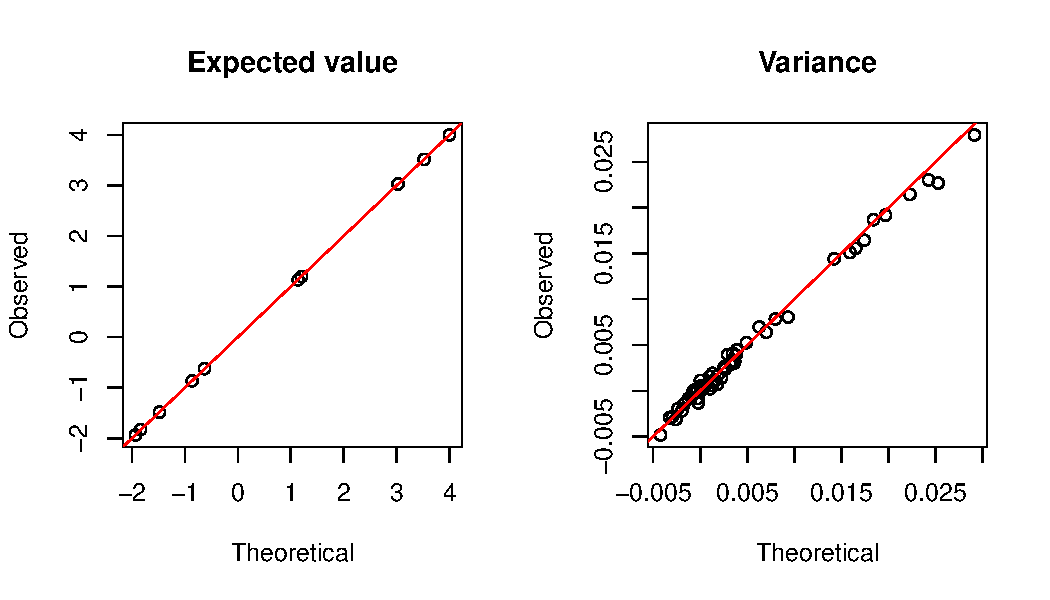
\includegraphics[width=\maxwidth]{figure/q6_graphs-1} \caption[Observed vs]{Observed vs. Theoretical Expectation and Variance for the fused ridge estimator}\label{fig:q6_graphs}
\end{figure}


\end{knitrout}




\end{document}
